%% Structure
%% Cambiar 'program' por 'project'
%% Tikz
%%% Tables --> 
\documentclass{article}
\usepackage{tikz}
\usetikzlibrary{arrows.meta, shapes.geometric, positioning}

\tikzset{
  >={Latex[length=2mm,width=2mm]},
  base/.style = {draw, minimum width=2.5cm, minimum height=1cm,
                 font=\sffamily, text centered, node distance=10mm},
}

\begin{document}
\begin{figure}[h]
    \centering
    \resizebox{\textwidth}{!}{%
        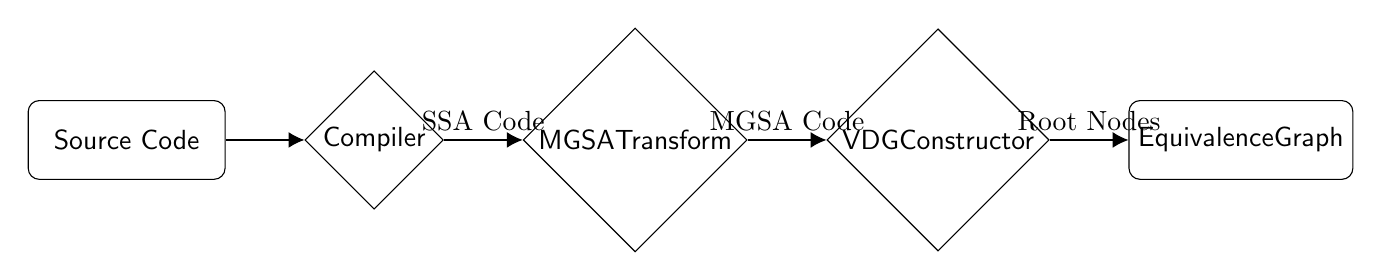
\begin{tikzpicture}[
            state/.style   = {base, rectangle, rounded corners},
            transform/.style = {base, diamond, minimum size=10mm, aspect=1, inner sep=1pt},
        ]
        \node[state]      (source)  {Source Code};
        \node[transform, right=of source] (compiler) {Compiler};
        \node[transform, right=of compiler] (mgsa) {MGSA\\Transform};
        \node[transform, right=of mgsa] (vdg) {VDG\\Constructor};
        \node[state, right=of vdg] (egraph) {Equivalence\\Graph};

        \draw[->] (source)   -- (compiler) node[midway,above] { };
        \draw[->] (compiler) -- (mgsa)     node[midway,above] {SSA Code};
        \draw[->] (mgsa)     -- (vdg)      node[midway,above] {MGSA Code};
        \draw[->] (vdg)      -- (egraph)   node[midway,above] {Root Nodes};

        \end{tikzpicture}%
        }
    \caption{Pipeline from source code to equivalence graph.}
\end{figure}

The project applies a set of transfomations onto the original C source file to facilitate the analysis done in the Equivalence Graph.
The first transform applied transforms the C code into LLVM intermediate representation, a simpler and more abstract represention.
One of the advantages of the LLVM representation is that it is written in a representation known as Single Static Assignment (SSA),
this representation guarantees that each variable is assigned exactly once, thus simplifying any kind of variable alias problem that may have arise if we were to use
the plain C code.
Once we have the LLVM representation we use the LLVM Compiler to pass it through the mem2reg pass, this transformation further simplifies the LLVM file
as it takes out a lot of unnecessary instructions and places $\phi$-nodes, this nodes are used in LLVM to solve merge conflict that may appear when assigning
to the same variable different values in different branches.
Then we extract the global variables and the functions from the final LLVM file. Each functions is extracted as its Control Flow Graph (CFG)
because in another transfomation we will use certain properties that this type of representation provides.

The second major transformation applied to the origin code is transitioning from SSA to a more complete representation called Monadic Gated SSA (MGSA).
As other papers mention this type of representation is \textbf{complete} and each instructions is \textbf{referencially transparent}.
We say that it is complete because all the information needed do the kind of analysis that we are doing can be found within said representation,
without the help of any other kind of representation. And by saying that each instruction is referencially transparent we are saying that
all of the information required to compute the value of an instruction is contained within the instruction.
The algorithm for this transformation is applied individually to each function definition of the C code. The algorithm is based in three different procedures.
First we traverse the CFG and look for instructions which should be modified, like alloc, load and $\phi$ instructions.
The second procedure transforms the low level instructions (the alloc, store and load instructions) into their monadic form, which is basically adding an arbitrary state
to each instruction that will be the output of the previous instruction.
The third procedure transforms all the $\phi$ instructions into $\gamma$ and $\mu$ instructions, and places $\eta$ instructions at the loop exit blocks.
$\gamma$ instructions are used in the merge blocks of various branching blocks, this instructions are represented as follows: $\gamma(Cond, TrueValue, FalseValue)$,
where the \textit{Cond} represents the condition that lead to the creation of the different branches, \textit{TrueValue} is the value assigned to the variable when the condition
evaluated to 'True' and \textit{FalseValue} represent the value coming from the false branch.
$\mu$ instructions are used in loop header block, they are represented as: $\mu(InitialValue, IterableValue)$. The \textit{InitialValue} is the value assigned to a variable
in the first iteration of the loop and \textit{IterableValue} is the value the variable will have in consecutive iterations.
Finally, the $\eta$ instructions placed at the exit blocks of a loop, are used to indicate the exit value of a variable declared within a loop, this are represented as $\eta(Cond, LoopValue)$.
\textit{Cond} is the loop condition and \textit{LoopValue} is the variable declared within the loop, this variables are the ones declared by the $\mu$ instructions.

The final transfomation turns the CFG into a Value Dependency Graph (VDG). This representation is the one used within the Equivalence Graph, its main advantage
over the CFG for the kind of analysis we are doing is that the VDG focuses on the data flow of the function, simplifying and refine the rules use for the analysis.
This transformation creates the VDG as an external representation of the Equivalence Graph and then we upload the root node of each VDG in the Equivalence Graph as this
nodes reach all the other nodes of the graph.
\end{document}
